\chapter{GPU Point Based Color Bleeding}

%-------------------------------------------------------------------------------
% SECTION: Algorithm Introduction
%-------------------------------------------------------------------------------
\section{Algorithm Introduction}

Indirect Illumination presents a computationally expensive problem. Potentially, the entirety of a scene's geometry could contribute illumination to any given point for which we try and compute indirect lighting. For Monte Carlo ray-tracing, intelligent randomness, spacial data structures, and attention to writing performant code can help alleviate the problem, but we can do better.

Our algorithm uses rasterization, rather than ray-tracing, to determine the radiance during the shading computation. Rasterization has traditionally been used in real-time graphics due its high throughput, but we can leverage that same throughput to reduce our time spent caculating indirect illumination. However, we want to also gain hardware acceleration, and GPU rasterization algorithms require specific input, namely triangles. Thus, we preprocess our scene geometry to convert it into a triangle-based surfel cloud, and store it in GPU memory. At render time, we can leverage the GPU to quickly rasterize these surfels, in parallel, onto cube-maps to capture the radiance at a point. In this way, each cube-map-pixel represents the radiance at the location of the cube-map, in the direction of that pixel. This is analogous to the way Monte Carlo ray-tracing casts a ray and calculates shading at its scene intersection to represent radiance, in the ray's direction, at the ray's origin.

In this chapter, we further discuss our GPU Point-Based Color Bleeding algorithm: section \ref{sec:surfel_generation} explains our preprocess for generating triangle-based surfels, section \ref{sec:rendering} follows with an explanation of our rendering pipeline. By combining our indirect illumination algorithm with GPU-hardware specifically designed for fast and parallel rasterization, we achieve quantitatively similar results in less time than Monte Carlo ray-tracing.

As an overview, the algorithm steps are as follows:

\begin{algorithm}[H]
\captionfont
\caption[GPU PBCB Algorithm]{Psuedocode for our GPU Point-Based Color Bleeding algorithm.}
\label{alg:gpu_pbcb}
{\fontsize{10}{9}\selectfont
\begin{algorithmic}
   \Function{GPUPointBasedColorBleeding}{$scene$}
      \ForAll{$geomPrimitive$ \textbf{in} $scene$}
         \State $surfels$ += GenerateSurfels($geomPrimitive$, 500) //see alg. \ref{alg:surfel_gen}
      \EndFor
      \State $rays$ := GenerateRays($scene$.imageDescription)
      \ForAll{$ray$ \textbf{in} $rays$}
         \State $intersection$ := Intersect($ray, scene$)
         \State $direct$ := DirectIllumination($intersection, scene$)
         \State $indirect$ := IndirectIllumination($intersection, scene$)
         \State $finalColor$ := $direct$ + $indirect$
         \State WriteColorToImage($ray, finalColor$)
      \EndFor
   \EndFunction
\end{algorithmic}
}
\end{algorithm}

%-------------------------------------------------------------------------------
% SECTION: Surfel Generation
%-------------------------------------------------------------------------------
\section{Surfel Generation}
\label{sec:surfel_generation}

The PBCB algorithm relies on the abstract representation of a scene's geometry as surfels in order to leverage the power of rasterization. Real-time graphics applications also utilize rasterization, but do not use surfel representations. This is because they target specific framerates between 30 and 60 frames per second, allowing 16 to 33 milliseconds for the computation of dynamic shadows, Lambertian shading, texture mapping, bump mapping, and other techniques on a per pixel basis. In the case of PBCB, rasterization must perform as fast as possible. To achieve this, additional computations of the kind referred to earlier (e.g. dynamic shadows) are avoided, and the rasterization algorithm simply uses the color of the surfel directly as the pixel's color. This is the reason why the PBCB algorithm does not simply rasterize the geometric primitives as a whole, but subdivides them into surfels with one color, computed as the direct illumination at the surfel's location on the scene geometry. If this were not the case, each geometric primitive would only be represented by one color, resulting in inaccurate indirect illumination.

In the traditional PBCB algorithm, surfels are disks, but our GPU PBCB cannot use this representation. The GPU is specifically designed to render images quickly by parallelizing the work, thus increasing throughput. However, we gain this performance at the cost of generality: the GPU can only process triangles as input data. Therefore, we must translate the representation of our geometric primitives into triangles (see Figure \ref{fig:surfelcloud}).

\begin{figure}[h!]
   \centering
   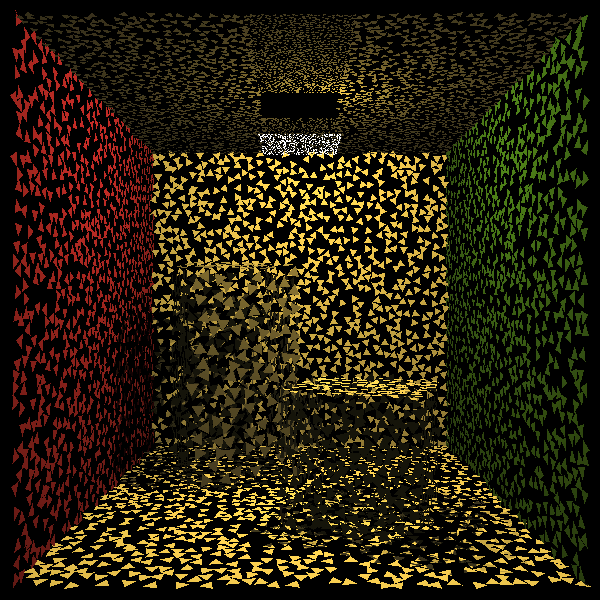
\includegraphics[width=100mm]{../img/cornell_simp_area_surfelcloud.png}
   \captionfonts
   \caption[Cornell Box with area light surfels]{The surfels generated for our Cornell Box with area light. Note that the surfel size has been reduced to exhibit the sufel shape and distribution.}
   \label{fig:surfelcloud}
\end{figure}

Each geometric primitive uses the same general algorithm to generate surfels, with differences in how the initial points are generated. We begin by generating a random distribution of points on the surface of the primitive, and use those points as the center for each triangular surfel. There has yet to be developed any algorithm with which to generate a uniformly random distribution of points on arbitrarily transformed geometry in linear time. In fact, [todo], [todo], and [todo] all require specific geometry that has not been transformed to generate a point distribution, and operate in polynomial time.

Our distribution algorithm is novel in its support for arbitrarily transformed geometry, but still requires polynomial time. However, because surfels are generated as a pre-process; the runtime does not affect our results. In general, we calculate our point distributions by first generating random points on the surface of our geometry, then pruning the two closest points repeatedly until we achieve the desired number of points. While in theory this algorithm does not achieve a mathematically uniform distribution, in practice it distributes the points well enough to achieve our goal of quantitatively similar results to Monte Carlo ray-tracing, is simple to understand and implement, and meets our requirement of supporting arbitrarily transformed geometry.

Once the points have been computed, the three triangle vertices are generated by adding the point's surface tangent vector to the point to solve for the first vertex, then rotating that vector by 120 degrees to solve for the second, and once more for the third. The length of the vector is determined by multiplying the distance between the two closest points and a constant. The goal is to have coverage over the surface of the geometry without superfluous gaps or overlaps. We have found that doubling the distance results in satisfactory coverage.

We discuss the general surfel generation algorithm in Section \ref{sec:surfel_gen}. We also discuss the specific point generation algorithms for boxes, spheres, and triangles in Section \ref{sec:point_gen}. In Section \ref{sec:surfel_gen} we discuss our algorithm for constructing traingular surfels, and in Section \ref{sec:VBOStorage} we discuss our storage method for these surfels.

% ---- SUBSECTION: Point Generation ----
\subsection{Point Generation}
\label{sec:point_gen}

In order to generate surfels for a any of our geometric primitives, we first generate a point distribution to act as center points for our surfels. The strategy we use for point distribution is stratified stochastic sampling.

% ---- SUBSUBSECTION: Box ----
\subsubsection{Box}
\label{sec:box_point_gen}
Points for the box primitive are generated per side. Each side is divided into a u-v grid, with a point for each intersection. We jitter the points to add randomness, which helps during the culling process explained later in this section, and to help mask any artifacting that can result from regular patterns. The pseudocode can be seen in Algorithm \ref{alg:box_point_gen}. Point distributions for a box can be seen in Figure \ref{fig:small_box_surfels}.

\begin{algorithm}
\captionfont
\caption[Box point generation]{Generate stratefied stochastic sample points for a box.}
\label{alg:box_point_gen}
{\fontsize{10}{9}\selectfont
\begin{algorithmic}
   \Function{SampleGeometry}{$box, numSamples$}
      \State $pointsPerSide := numSamples / 6$
      \State $pointsPerDim$ := sqrt($pointsPerSide$)
      \For{\textbf{each} $side$ \textbf{in} $boxSides$}
         \For{$u := 0...pointsPerDim$}
            \For{$v := 0...pointsPerDim$}
               \State $\alpha := (u + $rand($0,1$)$) / pointsPerDim$
               \State $\beta := (v + $rand($0,1$)$) / pointsPerDim$
               \If{$side$ = small z-plane}
                  \State $x := (1-\alpha) * box.start.x + \alpha * box.end.x$
                  \State $y := (1-\beta) * box.start.y + \beta * box.end.y$
                  \State $z := box.start.z$
               \ElsIf{$side$ = large z-plane}
                  \State $x := (1-\alpha) * box.start.x + \alpha * box.end.x$
                  \State $y := (1-\beta) * box.start.y + \beta * box.end.y$
                  \State $z := box.end.z$
               \ElsIf{$side$ = small x-plane}
                  \State $x := box.start.x$
                  \State $y := (1-\alpha) * box.start.y + \alpha * box.end.y$
                  \State $z := (1-\beta) * box.start.z + \beta * box.end.z$
               \ElsIf{$side$ = large x-plane}
                  \State $x := box.end.x$
                  \State $y := (1-\alpha) * box.start.y + \alpha * box.end.y$
                  \State $z := (1-\beta) * box.start.z + \beta * box.end.z$
               \ElsIf{$side$ = small y-plane}
                  \State $x := (1-\alpha) * box.start.y + \alpha * box.end.y$
                  \State $y := box.start.y$
                  \State $z := (1-\beta) * box.start.z + \beta * box.end.z$
               \ElsIf{$side$ = large y-plane}
                  \State $x := (1-\alpha) * box.start.y + \alpha * box.end.y$
                  \State $y := box.end.y$
                  \State $z := (1-\beta) * box.start.z + \beta * box.end.z$
               \EndIf
               \State $point := box.modelTransform *$ \textless$x, y, z$\textgreater
               \State $points$ += $point$
            \EndFor
         \EndFor
      \EndFor
      \State \Return $points$
   \EndFunction
\end{algorithmic}
}
\end{algorithm}

% ---- SUBSUBSECTION: Sphere ----
\subsubsection{Sphere}
\label{sec:sphere_point_gen}
Point generation for a sphere is based on a uniform sampling algorithm [TODO] that requires two uniform random variables as input. Instead of using entirely uniform random variables, u and v, we step through u and v coordinates, which effective subdivides the sphere into a grid. Again we jitter the coordinates to help randomize our surfel cloud.
The psuedocode can be seen in Algorithm \ref{alg:sphere_point_gen}.
Point distributions for a sphere can be seen in Figure \ref{fig:small_sphere_surfels}.

\begin{algorithm}[H]
\captionfont
\caption[Sphere point generation]{Generate stratefied stochastic sample points for a sphere.}
\label{alg:sphere_point_gen}
{\fontsize{10}{9}\selectfont
\begin{algorithmic}
   \Function{SampleGeometry}{$sphere, numSamples$}
      \State $numPointsU$ := sqrt($numSamples$)
      \State $numPointsV$ := $numSamples / numPointsU$
      \For{$i := 0...numPointsU$}
         \For{$j := 0...numPointsV$}
            \State $u := (i + $rand($0,1$)$) / numPointsU$
            \State $v := (j + $rand($0,1$)$) / numPointsV$
            \State $z := 1 - 2*u$
            \State $r$ := sqrt(max($0, 1- z*z$))
            \State $\phi := 2 * \pi * v$
            \State $x := r *$ cos($\phi$)
            \State $y := r *$ sin($\phi$)
            \State $point := \textless x, y, z \textgreater * sphere.radius + sphere.center$
            \State $point := sphere.modelTransform * point$
            \State $points$ += $point$
         \EndFor
      \EndFor
      \State \Return $points$
   \EndFunction
\end{algorithmic}
}
\end{algorithm}

% ---- SUBSUBSECTION: Triangle ----
\subsubsection{Triangle}
\label{sec:triangle_point_gen}
We generate our triangle sample points by modifying a uniform sample pattern algorithm [TODO] in a similar manner to our sphere point generation.
The original algorithm requires two uniformly random variables as input, and will generate a uniformly distributed random point on the triangle.
By discretizing the u and v values and stepping through them, we effectively walk a uniformly distributed grid across the triangle's surface area.
Again, we jitter the sample point location in order to eliminate any regular patterns.
The psuedocode can be seen in Algorithm \ref{alg:triangle_point_gen}.
Point distributions for a triangle can be seen in Figure \ref{fig:small_triangle_surfels}.

\begin{algorithm}[H]
\captionfont
\caption[Triangle point generation]{Generate stratefied stochastic sample points for a triangle.}
\label{alg:triangle_point_gen}
{\fontsize{10}{9}\selectfont
\begin{algorithmic}
   \Function{SampleGeometry}{$triangle, numSamples$}
      \State $numPointsU$ := sqrt($numSamples$)
      \State $numPointsV$ := $numSamples / numPointsU$
      \State $v_{0..1} := triangle.vertex1 - triangle.vertex0$
      \State $v_{0..2} := triangle.vertex2 - triangle.vertex0$
      \For{$i := 0...numPointsU$}
         \For{$j := 0...numPointsV$}
            \State $u := (i + $rand($0,1$)$) / numPointsU$
            \State $v := (j + $rand($0,1$)$) / numPointsV$
            \State // Inside or outside the triangle?
            \If{$u + v < 1$}
               \State $point := triangle.vertex0 + u*v_{0..1} + v*v_{0..2}$
            \Else
               \State $point := triangle.vertex0 + (1-u)*v_{0..1} + (1-v)*v_{0..2}$
            \EndIf
            \State $point := triangle.modelTransform * point$
            \State $points$ += $point$
         \EndFor
      \EndFor
      \State \Return $points$
   \EndFunction
\end{algorithmic}
}
\end{algorithm}

With the previous point distribution algorithms, we must address the issue of non-uniform scaling. For example, if we are generating points for a box scaled more in the y-axis than the x- or z-axis, then our computed sample points will be further spaced apart along that axis. This leaves us with a sampling pattern that is not uniform, but stretched in one direction.

Our solution to this problem is simple, easy to implement, and novel in the fact that it is geometry and transformation independent. We generate a multiple of the requested number of sample points, jitter their location, and repeatedly cull the two closest points until we arrive at the desired number of points. In this way, we work backwards to a more uniform distribution in a way that supports arbitrary geometric topology and transformations. Figures \ref{fig:small_box_surfels}, \ref{fig:small_sphere_surfels}, and \ref{fig:small_triangle_surfels} show the result of this process for varying multiples of the requested number of surfels; notice the coverage issues caused by not generating more than the requested number of surfels (e.g. Figure \ref{fig:box500s}).

The pseudocode is listed in Algorithm \ref{alg:point_gen}.

\begin{algorithm}
\captionfont
\caption[Create Points and Cull]{Create points and repeatedly cull one of the two closest points.}
\label{alg:point_gen}
{\fontsize{10}{9}\selectfont
\begin{algorithmic}
   \Function{GeneratePoints}{$geomPrimitive, numberOfSamples$}
      \State $points :=$ SampleGeometry($geomPrimitive$, $2*numberOfSamples$) //alg. \ref{alg:box_point_gen}, \ref{alg:sphere_point_gen}, \ref{alg:triangle_point_gen}
      \While{$points$.length $>$ $desiredNumPoints$}
         \State $minPointIndex :=$ FindAndRemoveClosestPoints($points$)
         \State $points$.remove($minPointIndex$)
      \EndWhile
      \State \Return $points$
   \EndFunction
\end{algorithmic}
}
\end{algorithm}

% ---- SUBSECTION: Surfel Generation ----
\subsection{Surfel Generation}
\label{sec:surfel_gen}

With the points generated, our surfel generation algorithm is quite simple: it consists of using the sample points as the center for triangular surfels. The question we must answer is what surface area will achieve adequate coverage of the source geometry. Too large of a surface area results in extending our surfel borders beyond the edges of our geometry as well as excessive surfel overlapping. Too small of a surface area results in gaps between surfels. Both of these issues will cause artifacts in our rendering by misrepresenting the source geometry.

Our algorithm uses the distance between the two closest sample points as the theoretical radius required for disk surfels to adequately cover the geometry. (In practice, we double this radius in order to ensure coverage.) In order for our triangle surfels to match this surface area, we extrapolate the length of the vector from triangle surfel center to equilateral vertex using Equation \ref{eqn:tri_dist}.

\begin{equation}
vectorLength = \sqrt{ \frac{ \pi * radius^2 }{ \sqrt{3} * \sin^2(60) } }
\label{eqn:tri_dist}
\end{equation}
~

However, the random jittering of sample points often results in initial sample points that are very close together. While the jittering produces the desired randomness, it also gives us too low an estimate of the required radius; the result of which can be seen in Figure \ref{fig:box500}. But the aforementioned point culling solution (see Section \ref{sec:point_gen}) also solves this problem. By culling the closest points, we create a more uniform distribution with less variance in the distance between adjacent sample points.

For typical surfel generation times per geometric primitive, see Table \ref{tbl:surf_gen_times}. In psuedocode, our surfel generation algorithm is listed in Algorithm \ref{alg:surfel_gen}. And Figure \ref{fig:surfel_cloud_simple} is a rendering of the raw surfel cloud in OpenGL without any lighting.

\begin{figure}
   \centering
   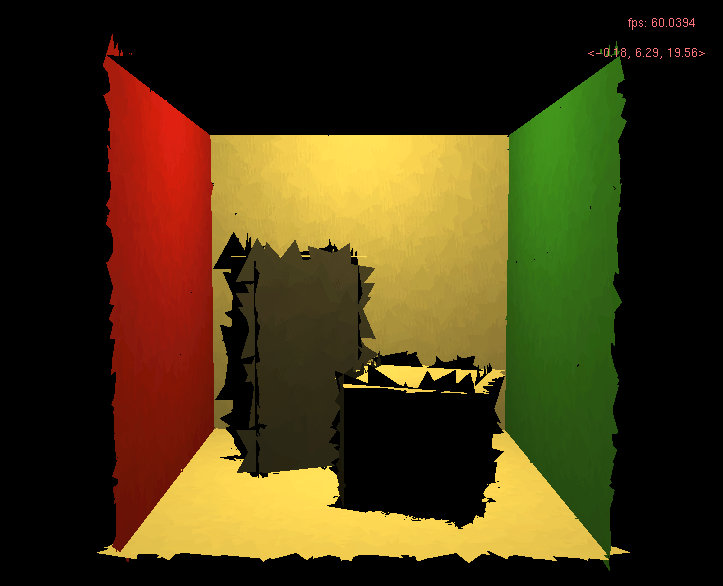
\includegraphics[width=100mm]{../img/surfel_cloud_simple.png}
   \captionfonts
   \caption[OpenGL Cornell Box surfel cloud]{Surfels generated for the Cornell Box scene rendered, without lighting, in OpenGL using a VBO.}
   \label{fig:surfel_cloud_simple}
\end{figure}

\begin{algorithm}[H]
\captionfont
\caption[Surfel generation]{Generate surfels from points on a geometric primitive.}
\label{alg:surfel_gen}
{\fontsize{10}{9}\selectfont
\begin{algorithmic}
   \Function{GenerateSurfels}{$geomPrimitive, numberOfSurfels$}
      \State $points :=$ GeneratePoints($geomPrimitive, numberOfSurfels$) //see alg. \ref{alg:point_gen}
      \State $minD :=$ FindClosestPoints($points$)
      \State $vectorLength := 2 * $sqrt(($PI * minD * minD$)$ / 1.299$) //see eqn. \ref{eqn:tri_dist}
      \ForAll{$point$ \textbf{in} $points$}
         \State $tangent :=$ CaculateTangent($point, geomPrimitive$)
         \State $surfel :=$ new surfel
         \State $surfel.v0 := point + vectorLength * tangent$
         \State $surfel.v1 := point + vectorLength * $rotate($tangent, 120$)
         \State $surfel.v2 := point + vectorLength * $rotate($tangent, 240$)
         \State $surfels$.add($surfel$)
      \EndFor
      \State \Return $surfels$
   \EndFunction
\end{algorithmic}
}
\end{algorithm}

\vfill
\begin{table}[h!]
   \centering
   \begin{tabular}{ | l | l | l | l | l | l | }
   \hline
   & 500 pts. & 1000 pts. & 2000 pts. & 4000 pts. & 8000 pts. \\ \hline
   Box & 1ms & 430ms & 5s 927ms & 43s 104ms & 6m 24s 819ms \\ \hline
   Sphere & 1ms & 714ms & 6s 274ms & 51s 286ms & 6m 50s 309ms \\ \hline
   Triangle & 1ms & 713ms & 6s 341ms & 51s 279ms & 6m 49s 847ms \\ \hline
   \end{tabular}
   \captionfonts
   \caption[Surfel generation times]{Surfel generation times listed by geometric primitive versus number of initial points.}
   \label{tbl:surf_gen_times}
\end{table}
\vfill
                        
\begin{figure}[h!]
   \centering
   \subfloat[500 points (1ms)]{\label{fig:box500s}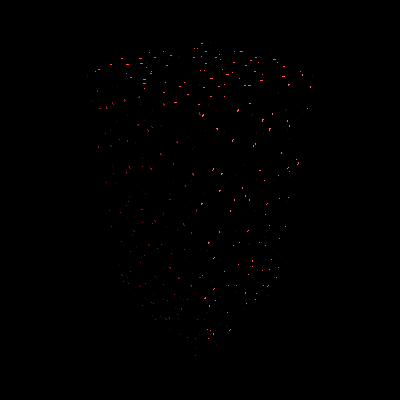
\includegraphics[width=50mm]{../img/box_500_initial_points_quarter_size_1ms.png}}
   ~
   \subfloat[1000 points (430ms)]{\label{fig:box1000s}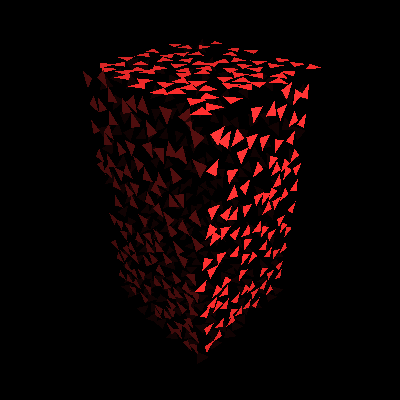
\includegraphics[width=50mm]{../img/box_1000_initial_points_quarter_size_430ms.png}}
   \\
   \subfloat[2000 points (5s 955ms)]{\label{fig:box2000s}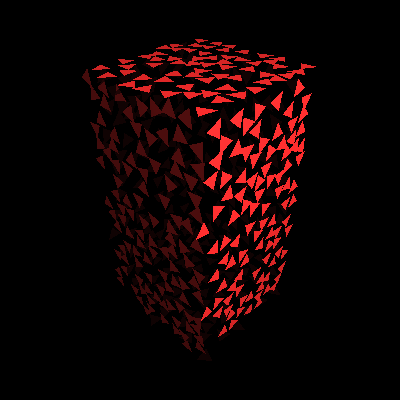
\includegraphics[width=50mm]{../img/box_2000_initial_points_quarter_size_5s955ms.png}}
   ~
   \subfloat[4000 points (43s 88ms)]{\label{fig:box4000s}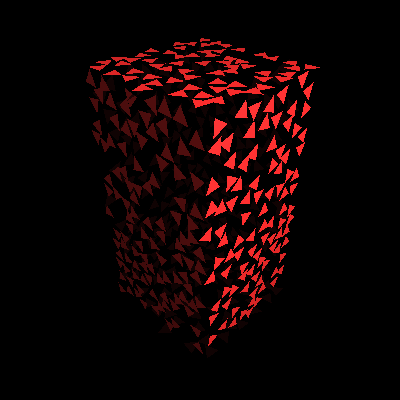
\includegraphics[width=50mm]{../img/box_4000_initial_points_quarter_size_43s88ms.png}}
   \\
   \subfloat[8000 points (6m 24s 803ms)]{\label{fig:box8000s}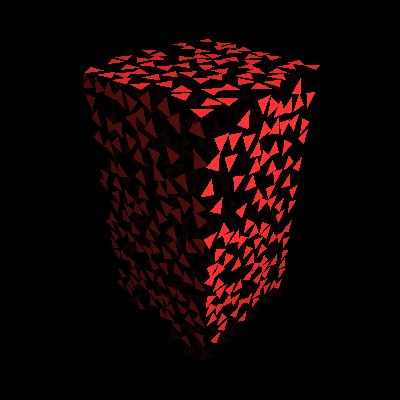
\includegraphics[width=50mm]{../img/box_8000_initial_points_quarter_size_6m24s803ms.png}}
   \captionfonts
   \caption[Box surfels at quarter size]{Surfel generation for a box, scaled in the y-axis, varying from 500 to 8000 initial points at quarter size. Generation times included in parenthesis.}
   \label{fig:small_box_surfels}
\end{figure}

\begin{figure}[h!]
   \centering
   \subfloat[500 points (1ms)]{\label{fig:box500}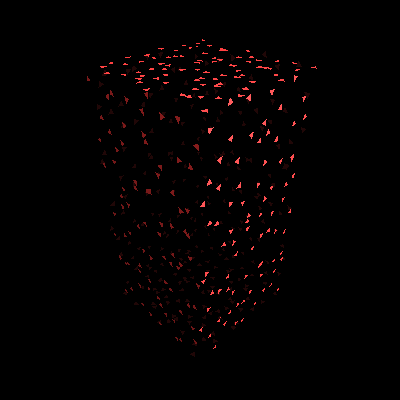
\includegraphics[width=50mm]{../img/box_500_initial_points_full_size_1ms.png}}
   ~
   \subfloat[1000 points (430ms)]{\label{fig:box1000}
\includegraphics[width=50mm]{../img/box_1000_initial_points_full_size_430ms.png}}
   \\
   \subfloat[2000 points (5s 927ms)]{\label{fig:box2000}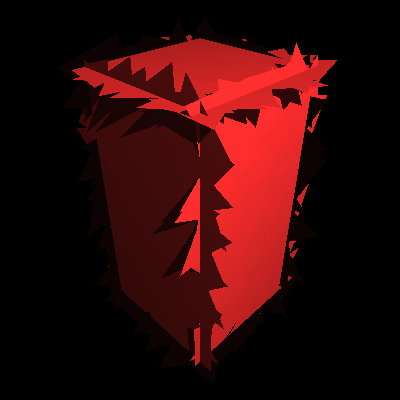
\includegraphics[width=50mm]{../img/box_2000_initial_points_full_size_5s927ms.png}}
   ~
   \subfloat[4000 points (43s 104ms)]{\label{fig:box4000}
\includegraphics[width=50mm]{../img/box_4000_initial_points_full_size_43s104ms.png}}
   \\
   \subfloat[8000 points (6m 24s 819ms)]{\label{fig:box8000}
\includegraphics[width=50mm]{../img/box_8000_initial_points_full_size_6m24s819ms.png}}
   \captionfonts
   \caption[Box surfels at full size]{Surfel generation for a box, scaled in the y-axis, varying from 500 to 8000 initial points at full size. Generation times included in parenthesis.}
   \label{fig:box_surfels}
\end{figure}

\begin{figure}[h!]
   \centering
   \subfloat[500 points (1ms)]{\label{fig:sphere500s}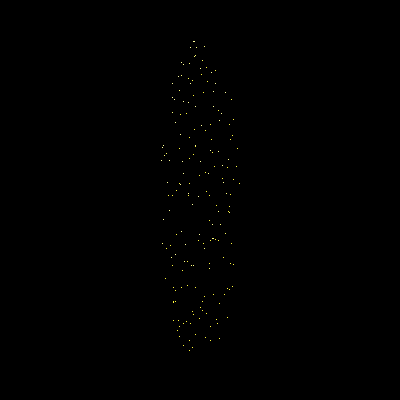
\includegraphics[width=50mm]{../img/sphere_500_initial_points_quarter_size_1ms.png}}
   ~
   \subfloat[1000 points (708ms)]{\label{fig:sphere1000s}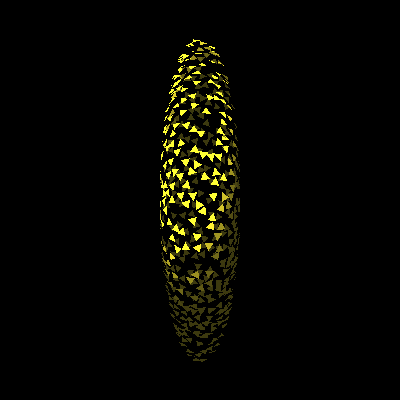
\includegraphics[width=50mm]{../img/sphere_1000_initial_points_quarter_size_708ms.png}}
   \\
   \subfloat[2000 points (6s 268ms)]{\label{fig:sphere2000s}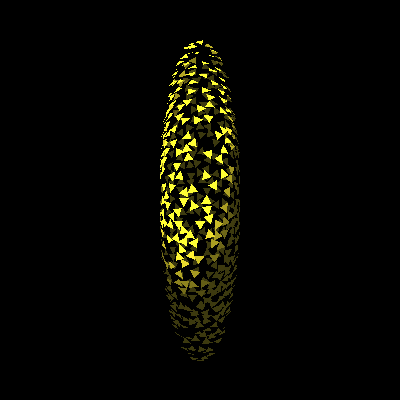
\includegraphics[width=50mm]{../img/sphere_2000_initial_points_quarter_size_6s268ms.png}}
   ~
   \subfloat[4000 points (51s 689ms)]{\label{fig:sphere4000s}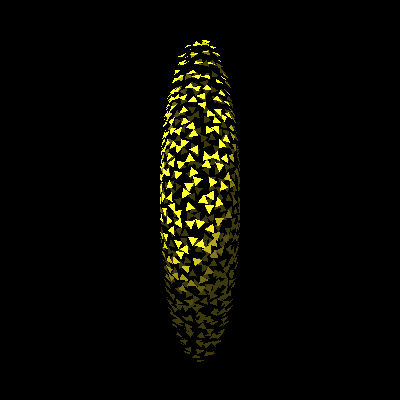
\includegraphics[width=50mm]{../img/sphere_4000_initial_points_quarter_size_51s689ms.png}}
   \\
   \subfloat[8000 points (6m 49s 391ms)]{\label{fig:sphere8000s}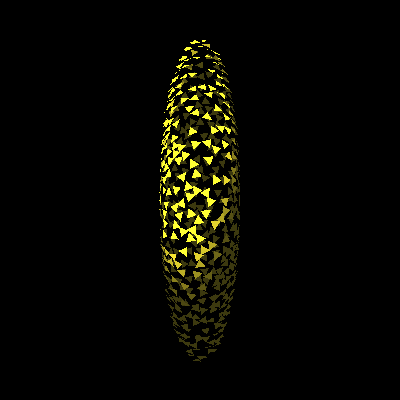
\includegraphics[width=50mm]{../img/sphere_8000_initial_points_quarter_size_6m49s391ms.png}}
   \captionfonts
   \caption[Sphere surfels at quarter size]{Surfel generation for a sphere, scaled in the y-axis, varying from 500 to 8000 initial points at quarter size. Generation times included in parenthesis.}
   \label{fig:small_sphere_surfels}
\end{figure}

\begin{figure}[h!]
   \centering
   \subfloat[500 points (1ms)]{\label{fig:sphere500}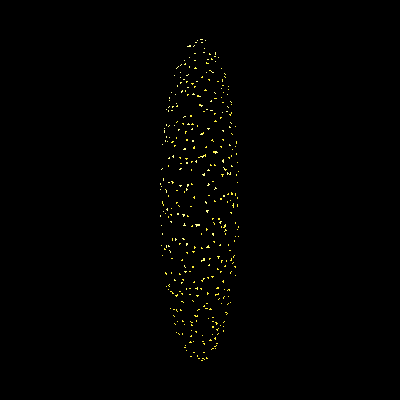
\includegraphics[width=50mm]{../img/sphere_500_initial_points_full_size_1ms.png}}
   ~
   \subfloat[1000 points (714ms)]{\label{fig:sphere1000}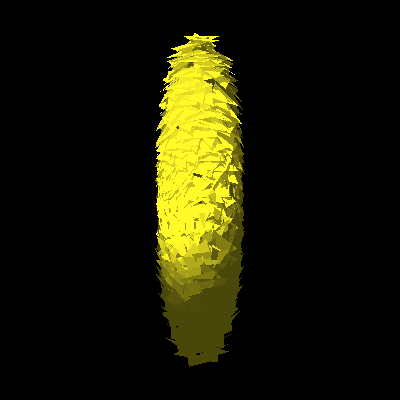
\includegraphics[width=50mm]{../img/sphere_1000_initial_points_full_size_714ms.png}}
   \\
   \subfloat[2000 points (6s 274ms)]{\label{fig:sphere2000}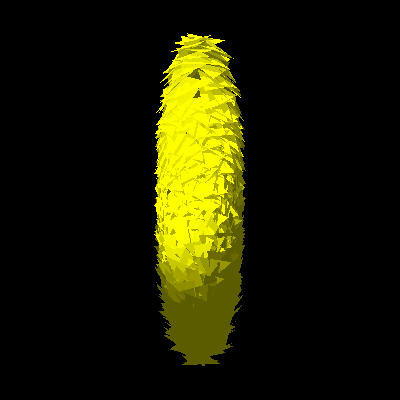
\includegraphics[width=50mm]{../img/sphere_2000_initial_points_full_size_6s274ms.png}}
   ~
   \subfloat[4000 points (51s 286ms)]{\label{fig:sphere4000}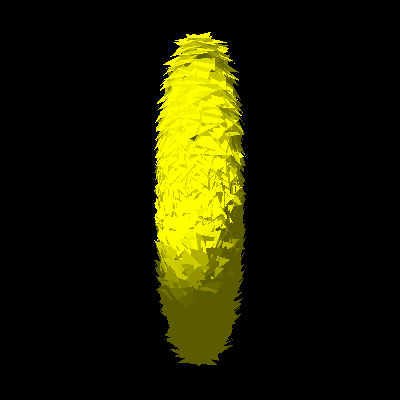
\includegraphics[width=50mm]{../img/sphere_4000_initial_points_full_size_51s286ms.png}}
   \\
   \subfloat[8000 points (6m 50s 309ms)]{\label{fig:sphere8000}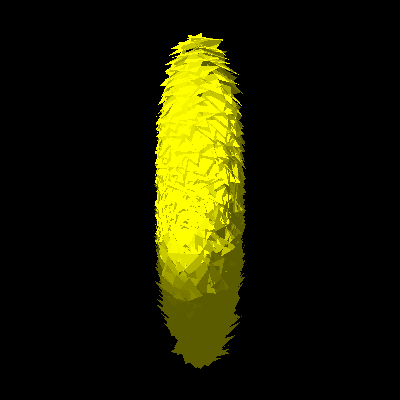
\includegraphics[width=50mm]{../img/sphere_8000_initial_points_full_size_6m50s309ms.png}}
   \captionfonts
   \caption[Sphere surfels at full size]{Surfel generation for a sphere, scaled in the y-axis, varying from 500 to 8000 initial points at full size. Generation times included in parenthesis.}
   \label{fig:sphere_surfels}
\end{figure}

\begin{figure}[h!]
   \centering
   \subfloat[500 points (1ms)]{\label{fig:tri500s}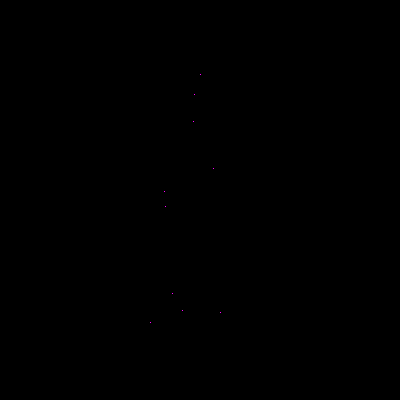
\includegraphics[width=50mm]{../img/triangle_500_initial_point_5xMinDist_1ms.png}}
   ~
   \subfloat[1000 points (703ms)]{\label{fig:tri1000s}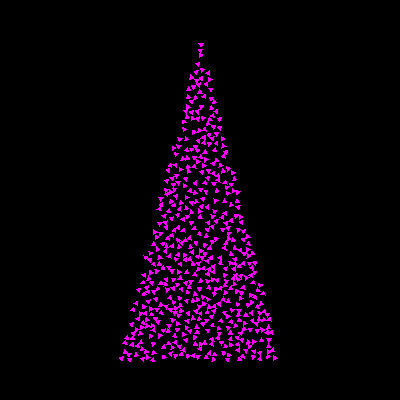
\includegraphics[width=50mm]{../img/triangle_1000_initial_point_5xMinDist_703ms.png}}
   \\
   \subfloat[2000 points (6s 283ms)]{\label{fig:tri2000s}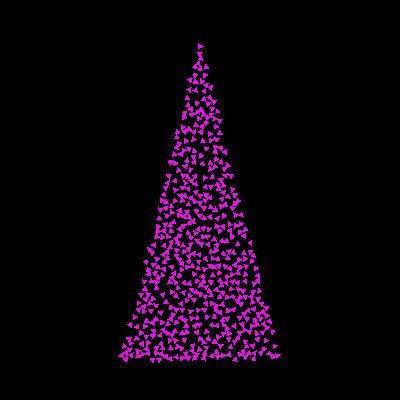
\includegraphics[width=50mm]{../img/triangle_2000_initial_point_5xMinDist_6s283ms.png}}
   ~
   \subfloat[4000 points (51s 432ms)]{\label{fig:tri4000s}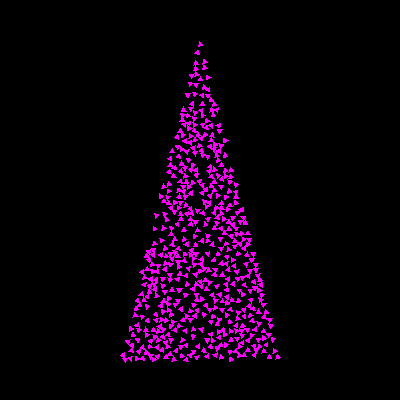
\includegraphics[width=50mm]{../img/triangle_4000_initial_point_5xMinDist_51s432ms.png}}
   \\
   \subfloat[8000 points (6m 49s 630ms)]{\label{fig:tri8000s}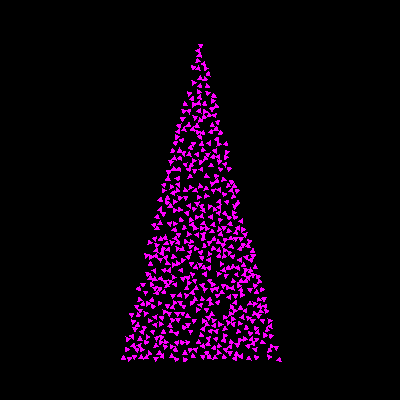
\includegraphics[width=50mm]{../img/triangle_8000_initial_point_5xMinDist_6m49s630ms.png}}
   \captionfonts
   \caption[Triangle surfels at quarter size]{Surfel generation for a triangle, scaled in the y-axis, varying from 500 to 8000 initial points at 1/4 size. Generation times included in parenthesis.}
   \label{fig:small_triangle_surfels}
\end{figure}

\begin{figure}[h!]
   \centering
   \subfloat[500 points (1ms)]{\label{fig:tri500}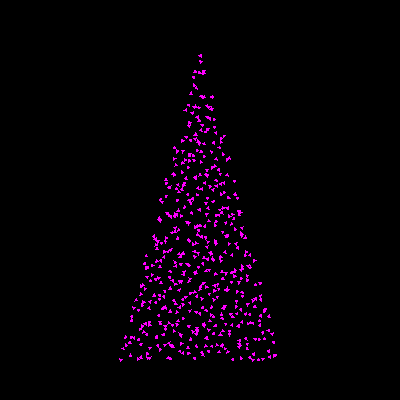
\includegraphics[width=50mm]{../img/triangle_500_initial_point_2xMinDist_1ms.png}}
   ~
   \subfloat[1000 points (713ms)]{\label{fig:tri1000}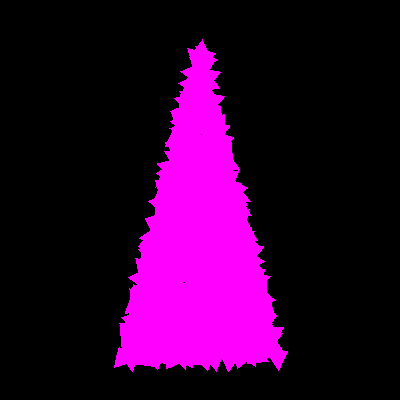
\includegraphics[width=50mm]{../img/triangle_1000_initial_point_2xMinDist_713ms.png}}
   \\
   \subfloat[2000 points (6s 341ms)]{\label{fig:tri2000}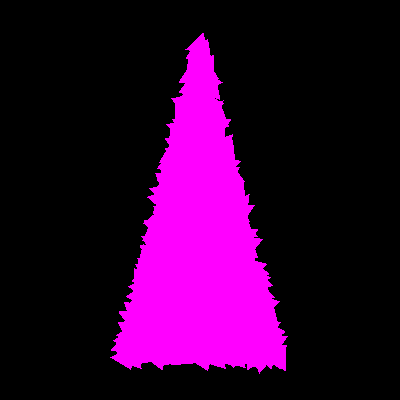
\includegraphics[width=50mm]{../img/triangle_2000_initial_point_2xMinDist_6s341ms.png}}
   ~
   \subfloat[4000 points (51s 279ms)]{\label{fig:tri4000}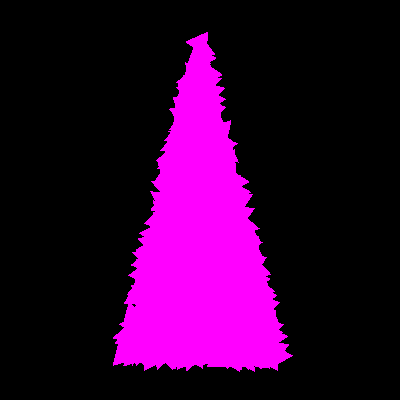
\includegraphics[width=50mm]{../img/triangle_4000_initial_point_2xMinDist_51s279ms.png}}
   \\
   \subfloat[8000 points (6m 49s 847ms)]{\label{fig:tri8000}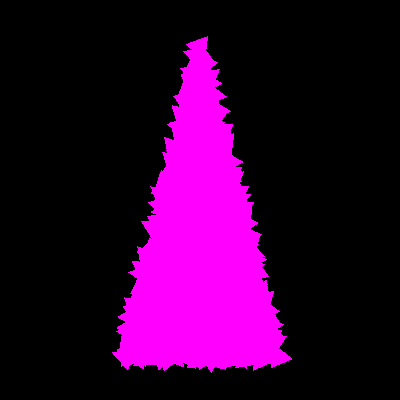
\includegraphics[width=50mm]{../img/triangle_8000_initial_point_2xMinDist_6m49s847ms.png}}
   \captionfonts
   \caption[Triangle surfels at full size]{Surfel generation for a triangle, scaled in the y-axis, varying from 500 to 8000 initial points at full size. Generation times included in parenthesis.}
   \label{fig:triangle_surfels}
\end{figure}

% ---- SUBSECTION: VBO Storage ----
\subsection{VBO Storage}
\label{sec:VBOStorage}

The surfels are generated on the CPU, but they must be rendered by the GPU. Therefore, it is logical to store them in GPU memory. This avoids the latency of transferring data over the CPU-to-GPU bus, which we discuss in Section \ref{sec:cpu_v_gpu}. For this purpose we leverage the OpenGL Vertex Buffer Object, or VBO. This data structure is an array of vertices paired with colors. Additionally, we never update the surfel vertex data, so we can store them on the GPU during our pre-process.

%-------------------------------------------------------------------------------
% SECTION: Rendering
%-------------------------------------------------------------------------------
\section{Rendering}
\label{sec:rendering}
Our rendering algorithm follows standard ray-tracing as discussed in Section \ref{sec:ray_tracing_intro} [TODO: possibly add a more in-detail section in background work], with the exception of the indirect lighting computation. The pseudocode is listed in Algorithm [TODO].

The indirect lighting computation uses our GPU PBCB algorithm and is the focus of this thesis. We describe the algorithm in detail in Section \ref{sec:indirect}, discuss the performance characteristics in Section TODO (add a section here, or in the results section?), analyze our results in Section \ref{sec:analysis}, and discuss future work in Section \ref{sec:future_work}.

% ---- SUBSECTION: Ray-Tracing ----
\subsection{Ray-Tracing}
\ref{sec:rendering_ray_tracing}
First, we generate a list of rays, one per pixel, by iterating over all final-image pixels. As input we require a virtual camera definition, which provides a world-space location and field of view characteristics such as width and height of the final image. A ray is composed of an origin point, inherited from the virtual camera's location, and direction, calculated as the vector between the origin and associated pixel's center.

We then iterate over the list of rays, tracing them against the scene geometry to calculate their intersection point. The intersection algorithms are based on [TODO, pbr] and [TODO, essntl mth fr gms].

Once we solve for the ray's intersection point with a geometric object, we calculate lighting. Because light calculations are additive [TODO], we can split the calculation into a direct and an indirect computation.

Our direct lighting calculation is quite simple: in the case of point lighting, we simply trace one shadow ray (see section TODO) and if the path to the light is unobstructed, then we calculate standard Lambertian shading (see section TODO), and in the case of area lighting we trace multiple shadow rays, in a uniform random distribution over the area light geometry, and scale the Lambertian shading by the percent of unobstructed rays.


% ---- SUBSECTION: Indirect Gather via Rasterization (GPU PBCB) ----
\subsection{Indirect Gather via Rasterization (GPU PBCB)}
\label{sec:indirect}
By using the GPU's ability to rasterize triangles, we capture the incoming radiance at a ray intersection point by rasterizing our surfel cloud onto five 8 by 8 pixel textures arranged into a cube about the point. The cube represents the hemisphere used in Section [TODO:background lighting eqn]. Using this technique, we attempt to realize a speedup over Monte Carlo ray-tracing as well as software-based PBCB. The psuedocode is listed in Algorithm [TODO].

Our implementation utilizes the OpenGL API, along with helper libraries: GLUT and GLEW. Therefore, as a preamble to the algorithm, we must initialize OpenGL. This requires creating the OpenGL rendering context and associated buffers, and setting some constant state. In our case, we require an 8 by 8 pixel color texture and depth texture, and a vertex buffer with which we store our surfel data. Lastly, we set the constant rendering state by disabling OpenGL lighting such that the color we calculate in the surfel generation preprocess will be used directly, and by binding our textures and buffers, which informs OpenGL on how to use each buffer (e.g. render to color texture, or where vertex, color, and surface normal data is per triangle in the VBO).

As discussed in Section \ref{sec:rendering_ray_tracing} and \ref{sec:ray_tracing_intro}, the geometry intersection for each ray is computed, and then lighting for that point is calculated. And because light is linear [TODO], we can calculate our indirect illumination separately from direct, and combine at a later time.

We begin our indirect illumination calculation for each intersection point by constructing five cameras that hold the render state required to rasterize each cube face. The cameras store their location, direction, up-vector, field of view, and near and far planes. The location for each camera is inherited from the intersection point. The direction is the intersection point's surface normal for the camera representing the top of the cube, and for the remaining cameras, we use the surface tangent, rotated in 90$^\circ$ increments. The up-vector for the cube-side cameras is the surface normal, and the top camera uses one of the side camera's direction vector. The field of view is set to 45$^\circ$ for each camera such that their viewing frustums fit together with no gaps (see figure [TODO]). The near plane is set to 0.01, and the far plane is set to 15 (see Section TODO), which we have found offers good results for our test scene.

Once the cube-face cameras are constructed, we iterate over each, and rasterize the surfel cloud onto an 8 by 8 pixel texture at the camera's near plane (see figure TODO). This texture data must then be read back from the GPU, and convolved into one indirect illumination value. We do this by iterating over each pixel, and adding it's contribution, calculated using the Lambertian reflectance model (see section TODO), to the final color.

Once each cube face has been rasterized and convolved, we return the final color as our indirect illumination value at the intersection point.

% ---- SUBSECTION: Final Color Computation ----
\subsection{Final Color Computation}

%-------------------------------------------------------------------------------
% SECTION: Review
%-------------------------------------------------------------------------------
\section{Review}

